\documentclass{article}

% Language setting
% Replace `english' with e.g. `spanish' to change the document language
\usepackage[brazil]{babel}

% Set page size and margins
% Replace `letterpaper' with `a4paper' for UK/EU standard size
\usepackage[letterpaper,top=2cm,bottom=2cm,left=3cm,right=3cm,marginparwidth=1.75cm]{geometry}
\usepackage[document]{ragged2e}
% Useful packages
\usepackage{amsmath}
\usepackage{graphicx}
\usepackage[colorlinks=true, allcolors=blue]{hyperref}
\usepackage{times}

\title{CONVERSÃO ENTRE FORMATOS DE REPRESENTAÇÃO DA ÁLGEBRA DE BOOLE}
\author{\\Erickson G. Müller\\mat: 20230001178}
\date{11 de abril de 2024}

\begin{document}
	\maketitle
	\vspace*{4cm}
	\section{Dado o circuito abaixo, apresente:}
		\hspace{1 cm}
		\includegraphics[scale=0.9]{Images/Circuito A.jpg}
		\pagebreak
		\subsection{Expressão Booleana:}
		\begin{equation*}
			X = \overline{\overline{\overline{A}.B}} +\overline{\overline{\overline{B}.\overline{C}}}+\overline{D}
		\end{equation*}
		
		\subsection{Tabela Verdade:}
		\hspace*{5 cm}
			\begin{tabular}{|c|c|c|c|c|}
			\hline
			\textbf{ A } & \textbf{ B } & \textbf{ C } & \textbf{ D } & \textbf{ X } \\
			\hline
			0 & 0 & 0 & 0 & 1 \\
			\hline
			0 & 0 & 0 & 1 & 1 \\
			\hline
			0 & 0 & 1 & 0 & 1 \\
			\hline
			0 & 0 & 1 & 1 & 0 \\
			\hline
			0 & 1 & 0 & 0 & 1 \\
			\hline
			0 & 1 & 0 & 1 & 1 \\
			\hline
			0 & 1 & 1 & 0 & 1 \\
			\hline
			0 & 1 & 1 & 1 & 1 \\
			\hline
			1 & 0 & 0 & 0 & 1 \\
			\hline
			1 & 0 & 0 & 1 & 1 \\
			\hline
			1 & 0 & 1 & 0 & 1 \\
			\hline
			1 & 0 & 1 & 1 & 0 \\
			\hline
			1 & 1 & 0 & 0 & 1 \\
			\hline
			1 & 1 & 0 & 1 & 0 \\
			\hline
			1 & 1 & 1 & 0 & 1 \\
			\hline
			1 & 1 & 1 & 1 & 0 \\
			\hline
			\end{tabular}
			\subsection{Expressão Booleana usando Maxtermos:}
			\begin{equation*}
				S = (A+B+\overline{C+D}).(\overline{A}+B+\overline{C+D}).(\overline{A+B}+C+\overline{D}).(\overline{A+B+C+D})
			\end{equation*}
		
		
	%\pagebreak
	\section{Dada a expressão booleana abaixo, apresente:}
		\begin{equation*}
			S = \overline{\overline{A} + B + \overline{CD}} + \overline{B}C\overline{D}
		\end{equation*}
		\subsection{Circuito:}
			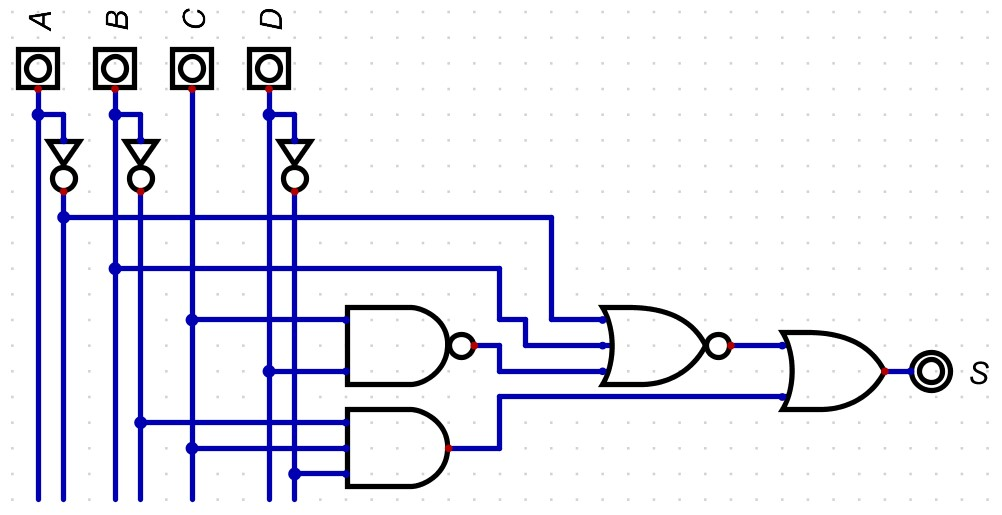
\includegraphics[scale=0.6]{Images/CIRCUITO B.jpg}
		\subsection{Tabela Verdade:}
		\hspace*{5 cm}
		\begin{tabular}{|c|c|c|c|c|}
			\hline
			\textbf{ A } & \textbf{ B } & \textbf{ C } & \textbf{ D } & \textbf{ S } \\
			\hline
			0 & 0 & 0 & 0 & 0 \\
			\hline
			0 & 0 & 0 & 1 & 0 \\
			\hline
			0 & 0 & 1 & 0 & 1 \\
			\hline
			0 & 0 & 1 & 1 & 0 \\
			\hline
			0 & 1 & 0 & 0 & 0 \\
			\hline
			0 & 1 & 0 & 1 & 0 \\
			\hline
			0 & 1 & 1 & 0 & 0 \\
			\hline
			0 & 1 & 1 & 1 & 0 \\
			\hline
			1 & 0 & 0 & 0 & 0 \\
			\hline
			1 & 0 & 0 & 1 & 0 \\
			\hline
			1 & 0 & 1 & 0 & 1 \\
			\hline
			1 & 0 & 1 & 1 & 1 \\
			\hline
			1 & 1 & 0 & 0 & 0 \\
			\hline
			1 & 1 & 0 & 1 & 0 \\
			\hline
			1 & 1 & 1 & 0 & 0 \\
			\hline
			1 & 1 & 1 & 1 & 0 \\
			\hline
		\end{tabular}
		\subsection{Expressão Booleana usando Mintermos:}
			\begin{equation*}
				S = (\overline{A.B}.C.\overline{D})+(A.\overline{B}.C.\overline{D})+(A.\overline{B}.C.D)
			\end{equation*}
		% A função é escrita na forma de uma Soma de Produtos (Mintermos), onde cada termo possui todas as variáveis (A, B e C) complementadas (negadas) ou não, ou na forma de um Produto de Somas (Maxtermos), onde cada fator contém a soma de todas as variáveis (complementadas ou não). Há uma exigência de que todas as variáveis devem aparecer em cada produto (no caso de mintermos) e em cada soma (no caso dos maxtermos).
		% MINTERMO - são termos somente com AND (termos PRODUTO). DEIXAR TUDO 1
		% MAXTERMO - são termos somente com OR (termos SOMA).	DEIXAR TUDO 0
		
		\section{A figura abaixo apresenta o diagrama de blocos de uma câmera fotográfica acionada por um controlador digital. A câmera possui 4 sensores (entradas) e dois atuadores (saídas).}
		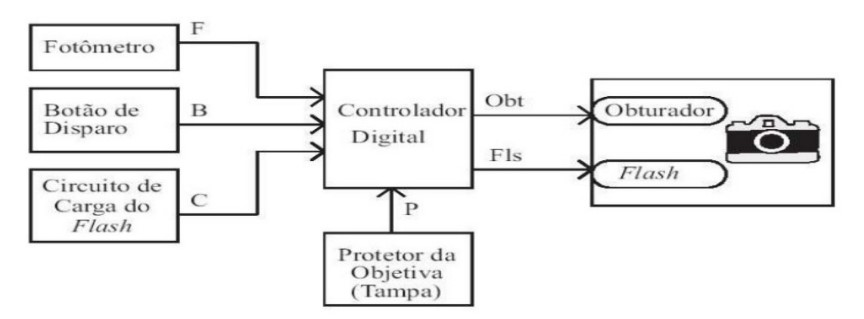
\includegraphics[scale = 0.6]{images/CAMERA.jpg}
		\\
		As entradas do controlador digital são: F – quantidade de Luz; C – carga para disparo do
		flash; B – botão de acionamento; P – presença da tampa. Os valores que as entradas podem
		assumir são apresentados na tabela abaixo:
		\\
		\vspace*{0.5cm}
		\hspace*{1cm}
		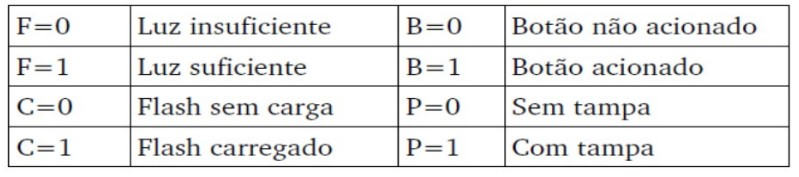
\includegraphics[scale = 0.65]{images/TABELA COND.jpg}
		\vspace*{0.5cm}
		\\
		As saídas a serem manipuladas pelo controlador digital são o Obturador (Obt) e o Flash (Fls).
		O Obturador é responsável pela abertura da luz natural na máquina e o Flash é responsável
		pela iluminação artificial do ambiente.\\
		Você ficou encarregado de projetar o controlador digital que contêm dois circuitos (um para
		cada saída, Obt e Fls).\\
		As regras de funcionamento são:\\
		1) O sistema só dispara quando o botão é pressionado.\\
		2) O Flash deve disparar quando não houver luz suficiente.\\
		3) Para o obturador acionar é necessário haver luz suficiente ou, quando não houver luz
		suficiente o flash deve estar carregado.\\
		4) O carregamento do flash começa imediatamente após o disparo e você não precisa se
		realizar nenhuma ação para isso.\\
		Com estas condições de operação e considerando os sensores disponíveis, apresente:\\
		\subsection{A tabela verdade para cada uma das saídas (obturador e flash);}
		\hspace*{1cm}
		\begin{tabular}{|c|c|c|c|c|}
			\hline
			\textbf{ F } & \textbf{ B } & \textbf{ C } & \textbf{ P } & \textbf{ Obt }\\
			\hline
			0 & 0 & 0 & 0 & 0 \\
			\hline
			0 & 0 & 0 & 1 & 0 \\
			\hline
			0 & 0 & 1 & 0 & 0 \\
			\hline
			0 & 0 & 1 & 1 & 0 \\
			\hline
			0 & 1 & 0 & 0 & 0 \\% - LUZ + BOTÃO - CARGA - PROTETOR = 0
			\hline
			0 & 1 & 0 & 1 & 0 \\% - LUZ + BOTÃO - CARGA + PROTETOR = 0
			\hline
			0 & 1 & 1 & 0 & 1 \\% - LUZ + BOTÃO + CARGA - PROTETOR = 1
			\hline
			0 & 1 & 1 & 1 & 0 \\% - LUZ + BOTÃO + CARGA + PROTETOR = 1
			\hline
			1 & 0 & 0 & 0 & 0 \\
			\hline
			1 & 0 & 0 & 1 & 0 \\
			\hline
			1 & 0 & 1 & 0 & 0 \\
			\hline
			1 & 0 & 1 & 1 & 0 \\
			\hline
			1 & 1 & 0 & 0 & 1 \\% + LUZ + BOTÃO - CARGA - PROTETOR = 1
			\hline
			1 & 1 & 0 & 1 & 0 \\% + LUZ + BOTÃO - CARGA + PROTETOR = 1 
			\hline
			1 & 1 & 1 & 0 & 1 \\% + LUZ + BOTÃO + CARGA - PROTETOR = 1
			\hline
			1 & 1 & 1 & 1 & 0 \\% + LUZ + BOTÃO + CARGA + PROTETOR = 1
			\hline
		\end{tabular}
		\hspace*{3cm}
		\begin{tabular}{|c|c|c|c|c|}
			\hline
			\textbf{ F } & \textbf{ B } & \textbf{ C } & \textbf{ P } & \textbf{ Fls }\\
			\hline
			0 & 0 & 0 & 0 & 0 \\%
			\hline
			0 & 0 & 0 & 1 & 0 \\%
			\hline
			0 & 0 & 1 & 0 & 0 \\%
			\hline
			0 & 0 & 1 & 1 & 0 \\%
			\hline
			0 & 1 & 0 & 0 & 0 \\% - LUZ + BOTÃO - CARGA - PROTETOR
			\hline
			0 & 1 & 0 & 1 & 0 \\% - LUZ + BOTÃO - CARGA + PROTETOR
			\hline
			0 & 1 & 1 & 0 & 1 \\% - LUZ + BOTÃO + CARGA - PROTETOR 1
			\hline
			0 & 1 & 1 & 1 & 0 \\% - LUZ + BOTÃO + CARGA + PROTETOR
			\hline
			1 & 0 & 0 & 0 & 0 \\%
			\hline
			1 & 0 & 0 & 1 & 0 \\%
			\hline
			1 & 0 & 1 & 0 & 0 \\%
			\hline
			1 & 0 & 1 & 1 & 0 \\%
			\hline
			1 & 1 & 0 & 0 & 0 \\% 
			\hline
			1 & 1 & 0 & 1 & 0 \\%
			\hline
			1 & 1 & 1 & 0 & 0 \\%
			\hline
			1 & 1 & 1 & 1 & 0 \\%
			\hline
		\end{tabular}
		\pagebreak
		\subsection{Os circuitos de acionamento do obturador e do flash.}
			\begin{equation*}
				%Obt = (\overline{F}.B.C.\overline{P})+(\overline{F}.B.C.P)+(F.B.\overline{C.P})+(F.B.\overline{C}.P)+(F.B.C.\overline{P})+(F.B.C.P)
				Obt = (\overline{F}.B.C.\overline{P})+(F.B.\overline{C.P})+(F.B.C.\overline{P})
			\end{equation*}
			\\
			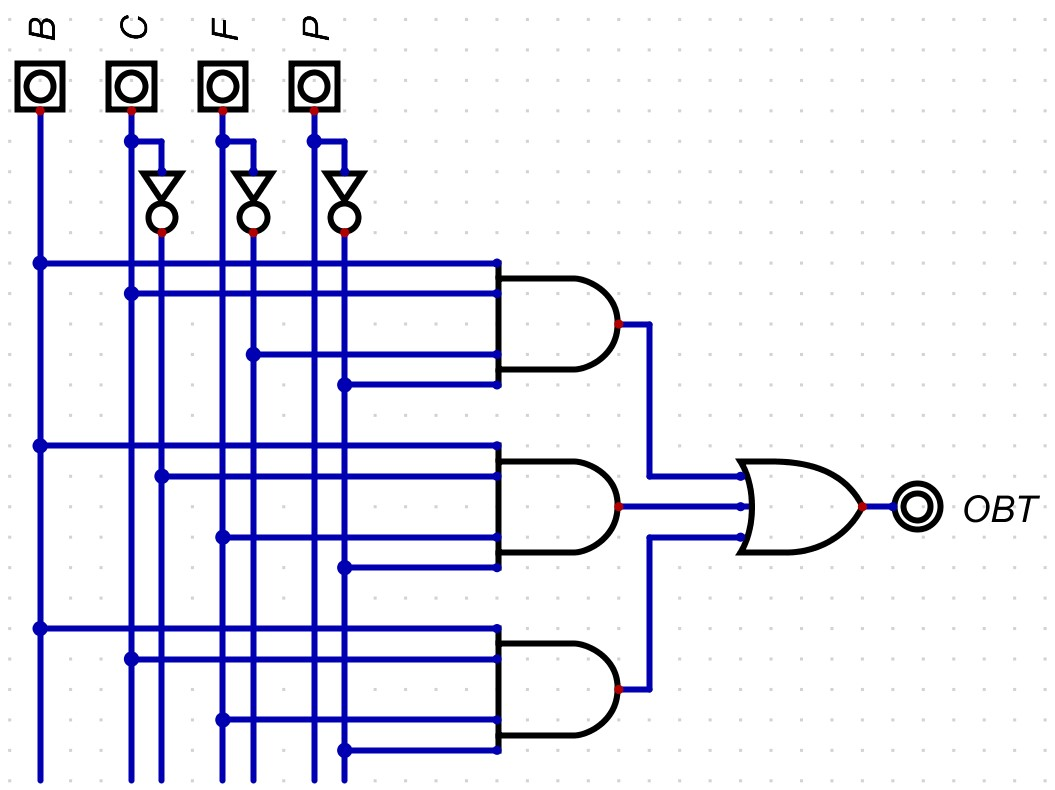
\includegraphics[scale=0.6]{images/OBT.jpg}
			\\
			\pagebreak
			\begin{equation*}
				Fls =
				(\overline{F}.B.C.\overline{P})
			\end{equation*}
			\\
			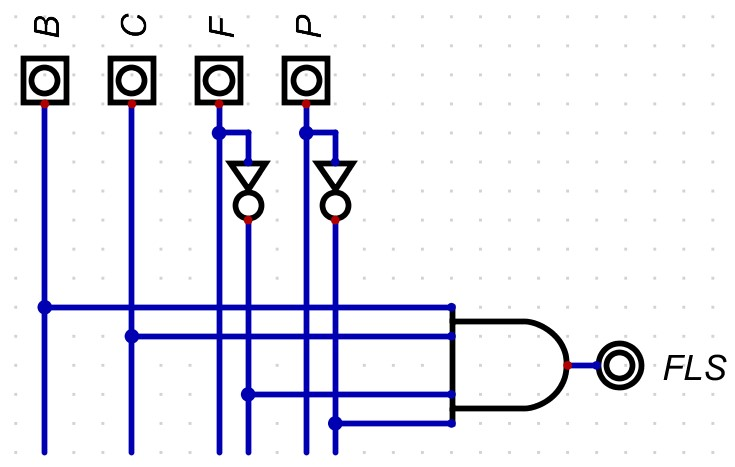
\includegraphics[scale=0.65]{images/FLS.jpg}

\end{document}